


\begin{figure}[b]
%\captionsetup[subfigure]{justification=centering}
\centering


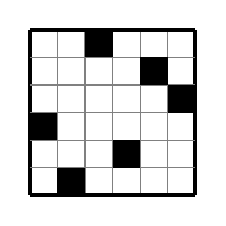
\begin{tikzpicture}[xscale=0.35, yscale=-0.35]
\draw[ultra thick] (0,0)--(0,6);
\draw[gray,thin] (1,0)--(1,6);
\draw[gray,thin] (2,0)--(2,6);
\draw[gray,thin] (3,0)--(3,6);
\draw[gray,thin] (4,0)--(4,6);
\draw[gray,thin] (5,0)--(5,6);
\draw[ultra thick] (6,0)--(6,6);

\draw[ultra thick] (0,0)--(6,0);
\draw[gray,thin] (0,1)--(6,1);
\draw[gray,thin] (0,2)--(6,2);
\draw[gray,thin] (0,3)--(6,3);
\draw[gray,thin] (0,4)--(6,4);
\draw[gray,thin] (0,5)--(6,5);
\draw[ultra thick] (0,6)--(6,6);

\fill [black] (2,0) rectangle (3,1);
\fill [black] (4,1) rectangle (5,2);
\fill [black] (5,2) rectangle (6,3);
\fill [black] (0,3) rectangle (1,4);
\fill [black] (3,4) rectangle (4,5);
\fill [black] (1,5) rectangle (2,6);

\end{tikzpicture}
%\caption{Costas array for $n=6$.}\label{fig:costas1}

\caption{An example Costas array}\label{fig:costas1}


\end{figure}


\begin{figure}[t]
\centering

%\vspace{-1cm}

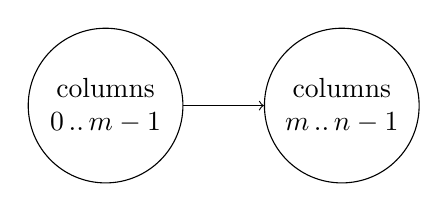
\begin{tikzpicture}
	\node [fill=white, draw=black, shape=circle, text width=1.5cm, text centered] (0) at (0, 0) {columns $0\, .. \, m-1$};
	\node [fill=white, draw=black, shape=circle, text width=1.5cm, text centered] (1) at (3, 0) {columns $m\, .. \, n-1$};
	\draw [fill=none, ->] (0) to (1);
\end{tikzpicture}
%\caption{DAG for Costas problem.}\label{fig:dag_example121}

\caption{A DAG decomposing Costas problem into two parts.}\label{fig:dag_example121}


%\caption{An example Costas array, and a DAG decomposing Costas problem into two parts.}\label{fig:costas_subfigure}\label{fig:dag_example121}\label{fig:costas1}
\end{figure}
